\documentclass[parskip=half]{scrartcl}
\usepackage[utf8]{inputenc}
\usepackage{relsize}
\usepackage{lmodern}
\usepackage[ngerman]{babel}
\usepackage{setspace}
\usepackage{hyperref}
\usepackage{graphicx}
\usepackage{listings}

\newcommand{\autoren}{Jan-Luca Gutsch, Sergej Frank, Valentin Beller, \\Marcel Schmidt, Jasmin Teller, Joshua Senkpiel}
\newcommand{\titel}{Bedienungsanleitung}
\newcommand{\untertitel}{Netzwerkplaner}
\newcommand{\Projekt}{Projekt 04}
\newcommand{\subnetcalc}{\textsc{Netzwerkplaner}}
\newcommand{\key}[1]{{\fontfamily{pcr}\selectfont #1}}
\newcommand{\ipAddress}[1]{{\fontfamily{pcr}\selectfont #1}}

\usepackage[automark,headsepline,ilines]{scrpage2}

\pagestyle{scrheadings}

% Kopfzeile
\ihead{\large{\textsc{\titel}}\\[2ex] \textit{\headmark}}
\chead{}
\ohead{}
\setlength{\headheight}{15mm}

% Fußzeile
\ifoot{\autoren}
\cfoot{}
\ofoot{\pagemark}

\onehalfspacing % Zeilenabstand 1,5 Zeilen
\frenchspacing % erzeugt ein wenig mehr Platz hinter einem Punkt

% Schusterjungen und Hurenkinder vermeiden
\clubpenalty = 10000
\widowpenalty = 10000
\displaywidowpenalty = 10000

\begin{document}

% Deckblatt
\begin{titlepage}
\begin{center}
\Large{\titel}\\[12ex]
\Large{\textbf{\untertitel}}\\[2ex]
\huge{\textbf{\Projekt}}\\[1.5ex]
\normalsize
Abgabetermin: Montag 12. Juni 2017\\[3em]
\textbf{Gruppenmitglieder:}\\
\autoren \\[5ex]
\end{center}
\end{titlepage}
\tableofcontents
\clearpage

\section{Einleitung}

\subsection{Überblick über die Software}
Die Software \subnetcalc\ hilft Ihnen Ihre Netzwerke effizient und sicher zu planen.

\subsection{Features}
Die Folgende Liste zeigt einen Auszug der Features der Software.
\begin{itemize}
    \item Erstellen von Netzwerken
    \item Erstellen von Subnetzwerken nach verschiedenen Kriterien
    \item Zuweisung von Hosts in Netzwerken mit Namensgebung
    \item Zuweisung von IPv6 Eigenschaften auf Netzwerke, Subnetzwerke und Hosts
    \item Speicher- und Ladeschnittstellen für die gesamte Planung oder einzelne Netzwerke
\end{itemize}
\section{Installation}
Befolgen Sie die folgenden Schritte um die Software \subnetcalc\ zu installieren.

\subsection{Voraussetzungen}

\subsubsection{Java}
Stellen Sie sicher, dass Sie Java auf Ihrem Gerät installiert haben. Für die
Ausführung von \subnetcalc\ ist mindestens die Version 1.8 in 32 oder 64 bit erforderlich.

\subsubsection{Betriebssystem}
Auf den folgenden Betriebssystemen wurde die Software erfolgreich getestet:
\begin{itemize}
    \item Windows 10
    \item Ubuntu 16.04
\end{itemize}

\textbf{Beachten Sie, dass die Software evtl. auch auf anderen Betriebssystemen
ordnungsgemäß funktioniert, jedoch kann dies nur für die oben genannten
garantiert werden.}

\subsection{Ausführung}
Um die Software auszuführen, befolgen Sie je nach Betriebssystem die folgenden
Schritte:

\subsubsection{Windows}
Um die Software zu starten öffnen Sie die Netzwerkplaner.jar Datei, die Sie
erhalten haben mit einem Doppelklick.

Alternativ navigieren Sie per Kommandozeile in den Ordner, der die
Netzwerkplaner.jar Datei enthält und führen Sie folgenden Befehl aus:

\begin{lstlisting}
    java -jar .\Netzwerkplaner.jar
\end{lstlisting}

\subsubsection{Ubuntu}
Verfahren Sie, wie für die Windows-Version, indem Sie im Dateimanager
die Netzwerkplaner.jar Datei per Doppelklick öffnen.

Alternativ navigieren Sie per Shell in den Ordner, der die
Netzwerkplaner.jar Datei enthält und führen Sie folgenden Befehl aus:

\begin{lstlisting}
    java -jar ./Netzwerkplaner.jar
\end{lstlisting}
\section{Grundlagen}

\subsection{Die Benutzeroberfläche}
Die folgende Abbildung zeigt die Benutzeroberfläche mit Beispieldaten.\\\\
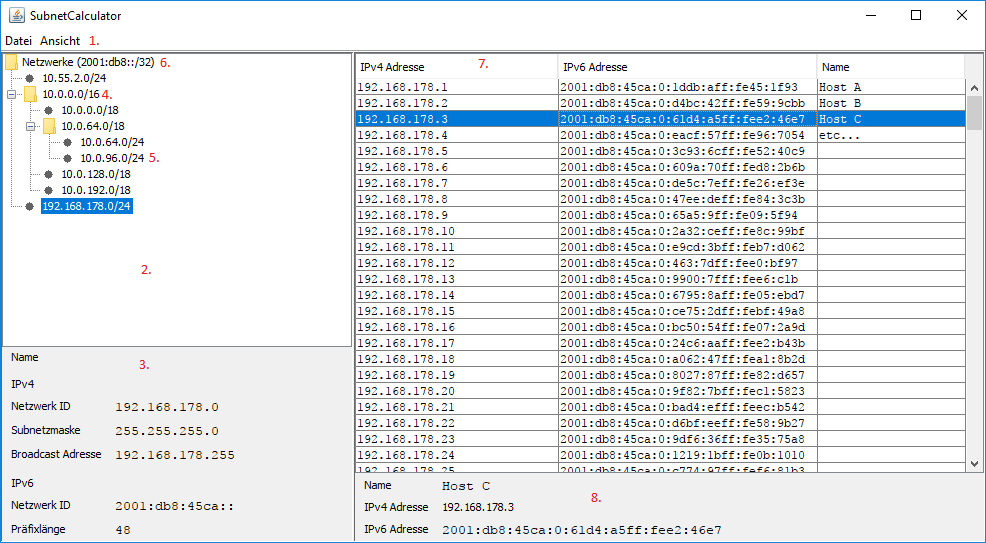
\includegraphics[width=\textwidth]{resources/oberflaeche.png}\\
\begin{enumerate}
    \item Menüleiste mit grundlegenden Funktionen
    \item Übersicht über alle Netzwerke und Subnetzwerke
    \item Details über das aktuell ausgewählte Netzwerk oder Subnetzwerke
    \item Ein Netzwerk
    \item Ein Subnetzwerk
    \item Globaler IPv6 Präfix
    \item Liste aller Hosts im aktuell ausgewählten Netzwerk
    \item Information über den aktuell ausgewählten Host
\end{enumerate}

\subsection{Funktionsweise}
Bei der Planung mit dem \subnetcalc\ werden grundlegend 3 Objekte unterschieden.

\subsubsection{Netzwerk}
Ein Netzwerk beschreibt ein Stammnetzwerk. Diese werden in der Oberfläche im
Netzwerkbaum direkt unter dem Punkt "`Netzwerke"' angezeigt.
Die Netzwerke liegen alle in einem logischen Stammnetzwerk mit der IPv4 Adresse
0.0.0.0/0. Daher dürfen sich die Netzwerke nicht überschneiden.

\subsubsection{Subnetzwerk, Subnetz}
Das Subnetzwerk, kurz Subnet, beschreibt ein Subnetzwerk eines Netzwerkes. Die
Subnetze eines Netzwerkes dürfen sich, wie die Netzwerke nicht überschneiden.
Subnetze können beliebig verschachtelt werden, wobei ein Subnetz entweder
weitere Subnetze oder Hosts enthalten darf.

Aus der technischen Sicht verhalten sich Netzwerke und Subnetzwerke gleich.
Daher wird im folgenden, wenn nicht anders beschrieben, nicht zwischen Netwerk
und Subnetzwerk unterschieden.

\subsubsection{Host}
Der Host beschreibt einen IP Endpunkt im Netzwerk, z.B. einen Computer. Hosts
liegen in einem  Netzwerk und haben immer eine zugewiesene IPv4 Adresse.
Wenn das Netzwerk mit IPv6 konfiguriert wurde, kann der Host auch eine IPv6
Adresse besitzen. Auch wenn bei der IPv6 Konfiguration in der Regel mehrere IPv6
Adressen pro Host oder Schnittstelle eingetragen werden, ist dies in dieser Software
nicht vorgesehen.

\subsection{Bedienung über das Kontextmenü}
Die meisten Bedienelemente sind in einem Kontextmenü enthalte, welches Sie über
einen Rechtsklick auf den Stammeintrag, ein Netzwerk oder ein Subnetz in der
Baumstruktur erreichen, oder auf einen Host in der Hosttabelle.
\section{Netzwerke}
Im folgenden wird der Umgang mit Netzwerken und ihrer Unterteilung in Subnetze
beschrieben.
Falls Sie die beschriebenen Kontextmenüeinträge nicht sehen können, stellen Sie sicher,
dass das Netzwerk noch keine Hosts enthält. Falls dies doch der Fall ist, entfernen Sie
diese, wie in \ref{AlleHostsEntfernen} beschrieben.

\subsection{Netzwerke anlegen}
\label{NetzwerkAnlegen}
Zum anlegen eines neuen Netzwerkes klicken Sie mit der rechten Maustaste auf den
Stammeintrag "`Netzwerke"'. Wählen sie im Kontextmenü den Menüpunkt
"`Neues Netzwerk"'. Bei fokusiertem Stammeintrag können Sie auch die
Tastenkombination \key{Strg+N} nutzen.
Es erscheint die Aufforderung die Netzwerk ID, sowie den Netzwerkpräfix anzugeben.
Alternativ können Sie auch die Netzwerkmaske angeben. Folgende Eingaben sind z.B.
möglich:

\ipAddress{10.5.0.0/24}\\
\ipAddress{192.168.178.0/255.255.255.0}

Achten Sie darauf, dass das eingegebene Netzwerk sich nicht mit bereits vorhanden
überschneidet. In diesem Falle erhalten Sie eine Fehlermeldung.

\subsection{Netzwerk in Subnetze teilen}
Die folgenden Punkte beschreiben Ihre Möglichkeiten Subnetze zu einem Netwerk
hinzuzufügen.

\subsubsection{Einzelnes Subnetz anlegen}
Zum anlegen eines einzelnen Subnetzes wählen sie im Kontextmenü des Netzwerkes den
Menüpunkt "`Neues Subnetz"'. Danach fahren Sie wie in \ref{NetzwerkAnlegen}
beschrieben fort.
Auch hier können Sie bei fokusiertem Netzwerk die Tastenkombination \key{Strg+N}
nutzen.

\subsubsection{Subnetz nach Anzahl der Hosts hinzufügen}
Wenn Sie die Anzahl der zu erwartenen Hosts in einem Subnetz kennen kann der
\subnetcalc\ ein möglichst kleines Subnetzwerk erstellen und es an der erstmöglichen
Position einfügen. Dafür gehen Sie wie folgt vor:

Wählen Sie im Kontextmenü des Netwerkes den Punkt "`Neues Subnetz nach Größe"' und tragen
Sie die Ihnen bekannte Anzahl an Hosts ein. Das neue Subnetzwerk wird automatisch erstellt 
und eingefügt.

\subsubsection{Netzwerke gleichmäßig in Subnetze teilen}
Sie können ein Netzwerk gleichmäßig in Subnetze teilen. Dafür stehen Ihnen zwei
Verfahren zur Verfügung: nach Größe und nach Anzahl.

\paragraph{Nach Größe}
Um ein Netzwerk nach der Größe der Subnetze zu teilen wählen Sie im Kontextmenü
des Netzwerkes den Menüpunkt "`Gleichmäßig nach Größe"'. Wählen Sie nun aus,
wie viele Hosts die Subnetze beinhalten sollen.

\paragraph{Nach Anzahl}
Um ein Netzwerk nach der Anzahl der Subnetze zu teilen wählen Sie im Kontextmenü
des Netzwerkes den Menüpunkt "`Gleichmäßig nach Anzahl"'. Wählen Sie nun aus, wie
in viele Subnetze das Netzwerk geteilt werden soll.

\textbf{Beachten Sie: Bei der gleichmäßigen Unterteilung eines Subnetzes werden alle
vorhandenen Subnetze überschrieben.}

\subsection{Netzwerk entfernen}
Um ein Netzwerk zu entfernen, wählen sie im Kontextmenü den Eintrag
"`Netzwerk/Subnetz löschen"', oder drücken Sie bei fokusiertem Netzwerk die
\key{Entfernen} Taste.

\subsection{Netzwerk unbenennen}
Sie können Netzwerken Namen geben. Um einem Netzwerk einen Namen zuzuweisen, oder
es umzubenennen, wählen Sie im Kontextmenü des Netwerkes den Menüpunkt
"`Umbenennen"'.
Wenn Sie den Namen eines Netzwerkes entfernen möchten, verfahren Sie genau so und lassen
Sie das Eingabefeld leer.
\section{Hosts}
Wenn ein Netzwerk keine weiteren Subnetze enthält können Sie die Hosts
konfigurieren. Im folgenden werden Ihre Möglichkeiten dazu gezeigt.
Falls Sie die beschriebenen Kontextmenüeinträge nicht sehen können, stellen
Sie sicher, dass dem Netzwerk keine weiteren Subnetze zugewiesen sind.

\subsection{Hosts hinzufügen}
\label{HostsHinzufuegen}
Um Hosts zu einem Netzwerk hinzuzufügen haben Sie 3 Möglichkeiten.

\textit{Falls Sie für das Netzwerk bereits IPv6 konfiguriert haben, können Sie
beim hinzufügen von Hosts automatisiert IPv6 Adressen zuweisen. Dabei handelt
es sich um zufällig generierte Adressen nach EUI Standard. Bestätigen Sie dafür
die entsprechende Sicherheitsabfrage.}

\subsubsection{Einzelnen Host hinzufügen}
Sie können einzelne Hosts mit oder ohne einer spezifischen IPv4 Adresse hinzufügen.

\subsubsection{Automatisch}
Wählen Sie im Kontextmenü des Netzwerkes den Menüpunkt "`Host hinzufügen"'.
Ein neuer Host mit der kleinstmöglichen IPv4 Adresse wird dem Netzwerk
hinzugefügt.

\subsubsection{Mit spezifischer IPv4 Adresse}
Um einen spezifischen Host hinzuzufügen wählen Sie im Kontextmenü des Netzwerkes
den Menüpunkt "`Host mit IPv4 Adresse hinzufügen"'.
Geben Sie nun die IPv4 Adresse an und bestätigen Sie diese.

\subsection{Alle Hosts hinzufügen}
Sie können ein Netzwerk mit allen möglichen Hosts füllen. Wählen Sie dazu den
Menüpunkt "`Alle Hosts hinzufügen"' im Kontextmenü des Netzwerkes aus.
Bereits konfiguriert Hosts bleiben erhalten.

\subsection{Hosts entfernen}
Falls Sie einen Host entfernen, oder dem Netzwerk Subnetze hinzufügen wollen,
befolgen Sie einen der nachfolgenden Schritte.

\subsubsection{Alle Hosts entfernen}
\label{AlleHostsEntfernen}
Wählen Sie den Menüpunkt "`Alle Hosts entfernen"' im Kontextmenü eines Netzwerkes
um alle Hosts des Netzwerkes zu entfernen. Nach dieser Operation, können Sie
dem Netzwerk wieder Subnetze hinzufügen.

\subsubsection{Einzelnen Host entfernen}
Um einen einzelnen Host zu entfernen klicken Sie mit der rechten Maustaste auf
den Host in der Host Tabelle um das Kontextmenü zu öffnen. Wählen sie den
Menüpunkt "`Host entfernen"' und bestätigen Sie die Sicherheitsabfrage.

Sie können diese Operation auch auf mehrer Hosts gleichzeitig ausüben. Markieren
Sie die Hosts, die gelöscht werden sollen, und wählen Sie den entsprechenden
Eintrag im Kontextmenü.

\subsection{Host bearbeiten}
\label{HostBearbeiten}
Sie können die IPv6 Adresse und den Namen eines Hosts bearbeiten. Gehen Sie
dafür wie folgt vor:\\
Klicken Sie doppelt auf die Zelle in der Host Tabelle, die
Sie ändern wollen, oder stellen Sie sicher, dass die Zelle, die Sie ändern
wollen im Fokus liegt und tippen Sie den neuen Wert ein.

\textbf{Beachten Sie, dass Sie die IPv4 Adresse eines Hosts nicht bearbeiten können.
Um die IPv4 Adresse eines Host zu ändern, fügen Sie einen neuen Host mit der
neuen IPv4 Adresse hinzu und übertragen Sie die Daten.}
\section{IPv6}
Der \subnetcalc\ unterstützt das Internet Protokoll in der Version 6.

\subsection{Globaler IPv6 Präfix}
Bei der Planung wird ein globaler IPv6 Präfix genutzt. Dieser ist optional und
kann z.B. einen Präfix repräsentieren, den Sie von Ihrem Internet Provider
erhalten haben.
Beim Start der Software ist der globale IPv6 Präfix auf \ipAddress{2001:db8::/32}
gesetzt. 

\subsubsection{Globalen Präfix anlegen}
\label{IPv6GlobalZuweisen}
Den globalen IPv6 Präfix können Sie anlegen, oder bearbeiten indem Sie das
Kontextmenü des Stammeintrages "`Netzwerke"' aufrufen und den Menüpunkt
"`Globalen IPv6 Präfix hinzufügen"' oder "`Globalen IPv6 Präfix bearbeiten"'
auswählen. geben Sie eine gültige IPv6 Netzwerk ID sowie eine IPv6 Präfixlänge
an. Stellen Sie sicher, dass alle IPv6 konfigurierten Netzwerke im
angegebenen IPv6 Präfix liegen.
Beispielhaft wären folgende Eingaben gültig:\\
\ipAddress{2001:db8:3b::/48}\\
\ipAddress{c11:29ad:0:49bf::/64}

\subsubsection{Globalen Präfix entfernen}
Um den Globalen IPv6 Präfix zu entfernen, rufen Sie das Kontextmenü des
Stammeintrages auf und wählen Sie den Menüpunkt "`Globalen IPv6 Präfix entfernen"'.
Alle IPv6 konfigurierten Netzwerke behalten ihre IPv6 Konfiguration.

\subsection{IPv6 in Netzwerken}
Um Netzwerke mit IPv6 zu konfigurieren gehen Sie wie folgt vor:

\subsubsection{IPv6 für Netzwerk konfigurieren}
Stellen Sie zunächst sicher, dass ein evtl. vorhandenes übergeordnetes Netzwerk
eine IPv6 Konfiguration besitzt. Anschließend wählen Sie den Menüpunkt
"`IPv6 zuweisen"' order "`IPv6 bearbeiten"' im Kontextmenü des Netzwerkes und
fahren Sie wie in \ref{IPv6GlobalZuweisen} beschrieben fort.

Sollte das Netzwerk bereits Hosts besitzen, können Sie allen Hosts eine zufällige
IPv6 Adresse zuweisen. Bestätigen Sie dafür die entsprechende Abfrage mit \key{Ja}.

\subsubsection{IPv6 aus Netzwerk entfernen}
Wenn Sie die IPv6 Konfiguration von einem Netzwerk entfernen wollen,
wählen sie den Menüpunkt "`IPv6 entfernen"' im Kontextmenü des Netzwerkes.
Beachten Sie, dass anders als beim globalen IPv6 Präfix auch alle Subnetzwerke
und Hosts ihre IPv6 Konfiguration verlieren.

\subsection{IPv6 Adressen fpr Hosts}
Um Hosts für IPv6 zu konfigurieren, muss zuerst das Netzwerk eine IPv6 Konfiguration besitzen.

\subsubsection{IPv6 Adresse zu Hosts hinzufügen}
\label{HostIPv6Hinzufuegen}
Wie bereits in \ref{HostBearbeiten} beschrieben, können Sie die IPv6 Adresse eines Hosts
durch die Hosttabelle ändern.
Stellen Sie sicher, dass eine eingegebene IPv6 Adresse im Bereich des Netzwerkes liegt und
noch nicht vergeben ist.

Alternativ können Sie auch für einen order mehrere Hosts automatisiert IPv6 Adressen
vergeben lassen. Markieren Sie dafür die Hosts in der Tabelle und wählen Sie im Kontextmenü
den Menüpunkt "`Zufällige IPv6 Adresse zuweisen"'.

\subsubsection{IPv6 Adresse von Host entfernen}
Um die IPv6 Adresse von einem Host zu entfernen, gehen Sie vor wie in
\ref{HostIPv6Hinzufuegen} beschrieben und lassen Sie die Tabellenzelle leer.
\section{Ansicht}
Sie können die Darstellung von IPv4 und IPv6 Adressen anpassen.
Die im folgenden genannten Menüpunkte finden Sie im Menü "`Ansicht"'.

\subsection{IPv4 Darstellung}
Wählen Sie im Menüpunkt "`Schreibweise IPv4"' die gewünschte Notationsweise.

\begin{description}
    \item[Dezimal] \ipAddress{192.168.178.28}
    \item[Binär] \ipAddress{11000000 10101000 10110010 00011100}
\end{description}

\subsection{IPv6 Darstellung}
Wählen Sie im Menüpunkt "`Schreibweise IPv6"' die gewünschte Notationsweise.

\begin{description}
    \item[Hexadezimal] \ipAddress{2001:db8:fe55:0::ca:39a}
    \item[Binär] \ipAddress{00100000 00000001 00001101 10111000 11111110 01010101
    00000000 00000000 00000000 00000000 00000000 00000000 00000000 11001010 00000011 10011010}
\end{description}
\section{Speichern und Laden}
Sie können eine Planung mit allen Netzwerken speichern und später wiederverwenden.
Alternativ können Sie auch einzelne Netzwerke exportieren und diese später in eine
andere Planung importieren.

\subsection{Netzwerke}
Die folgende Schritte beschreiben den Ex- und Import von einzelnen Netzwerken.

\subsubsection{Exportieren}
Um ein Netzwerk zu speichern, wählen Sie den Menüpunkt "`Speichern unter..."' im
Kontextmenü des Netzwerkes aus. Geben Sie einen Dateinamen und Speicherort ein und
speichern sie das Netzwerk.

Die gespeicherte Version eines Netzwerkes enthält alle Subnetzwerke und Hosts.

\subsubsection{Importieren}
Um ein Netzwerk zu importieren, wählen Sie zunächst das Netzwerk zu dem das zu
importierende Netzwerk hinzugefügt werden soll aus. Dabei kann es sich auch um
den Stammeintrag handeln. Nutzen Sie nun den Menüpunkt "`Netzwerk laden"' im
Kontextmenü und wählen Sie die Datei aus.

Stellen Sie sicher, dass das zu importierende Netzwerk in das übergeordnet
Netzwerk passt und es zu keinen Überscheidungen kommt.

\subsection{Planung}
Um Ihre gesamte Planung, inklusive aller Netzwerke abzuspeichern gehen Sie wie folgt
vor:

\subsubsection{Speichern}
Klicken Sie im Menü auf den Menüpunkt "`Datei"' und anschließend auf
"`Speichern unter..."'. Wähle Sie einen Dateinamen und einen Speicherort aus und
speichern Sie die Planung.

Die gespeicherte Verion der Planung enthält alle Netzwerke, ihre
Subnetzwerke und Hosts, sowie die globale IPv6 Konfiguration.

\subsubsection{Öffnen}
Um eine vorher gespeicherte Planung zu öffnen, wählen Sie im Menü den Menüpunkt
"`Datei"' und anschließend "`Öffnen"' aus. Wählen Sie die Datei und öffnen Sie
diese.

\textbf{Beachten Sie, dass beim Öffnen einer Planung die geöffnete Planung verworfen wird.
Speichern Sie diese bei Bedarf zuerst ab.}
\section{Quellcode}
Falls Sie Interesse am Quellcode der Software haben, steht dieser unter
MIT Lizenz auf GitHub zur Verfügung.
\url{https://github.com/SergejFrank/IT5LSubnetting}

\end{document}